\chapter{Data Model}\label{ch:datamodel}

\figref{fig:datamodel} shows the analysis classes of the data model used by the
application.

\begin{figure}[htb]
	\centering
	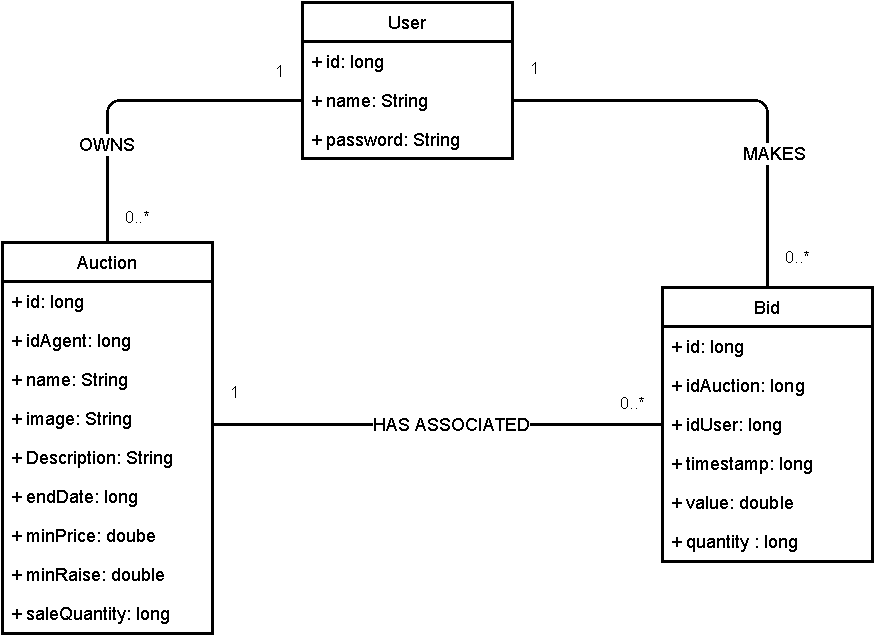
\includegraphics[width=\textwidth]{datamodel}
	\caption{Data model UML diagram (analysis classes)}\label{fig:datamodel}
\end{figure}

\begin{description}
	\item[User] A registered user:
		\begin{description}
			\item[id] Unique id of a user.
			\item[name] The username of a user.
			\item[password] The password of a user.
		\end{description}
	\item[Auction] An auction of the system:
		\begin{description}
			\item[Id] unique id of an auction.
			\item[IdAgent] id of the user that make the auction.
			\item[Name] name of the item of the auction.
			\item[Image] image of the items of the auction.
			\item[Description] description of the items of the auction.
			\item[EndDate] the date and time when the auctions ends.
			\item[MinPrice] starting price for each item of the bid.
			\item[MinRaise] minimum raise for each new bid.
			\item[SaleQuantity] number of items to sell.
		\end{description}
	\item[Bid] A bid for an auction made by a user:
		\begin{description}
			\item[Id] unique id of a bid.
			\item[IdAuction] id of the auction.
			\item[IdUser] id of the user that made the bid.
			\item[Timestamp] timestamp the bid was made.
			\item[BidValue] value of the bid for single item.
			\item[Quantity] number of items you want to buy.
		\end{description}
\end{description}
